% !TeX root = ../main.tex
% Add the above to each chapter to make compiling the PDF easier in some editors.

\chapter{Background}\label{chapter:background} % Anshul 4 sayfa yazmış

\section{Who uses Cloud ?} % Cloud usage scenarios
Cloud computing becomes more and more widespread as it's capabilities for on-demand provisioning and support for different use cases increases. Currently cloud computing is being used in many different aspects of our life. \cite{cloud-use-cases} Some of those aspects include file storage like OneDrive, database as a service systems like Amazon SimpleDB, entertainment services such as Netflix, multiplayer online games like Dota 2. Businesses are also using cloud computing for instant messaging between departments through applications like Slack or storing customer data in customer relationship management services provided by companies such as SAP or Salesforce. Many businesses also offload their computing requirements to cloud for data mining or for project management, as the Pay-per-use model of cloud is very beneficial for companies because they don't need to maintain a cluster of computers in premise. Cloud computing is also being used to host massive websites such as Facebook.com or Amazon.com.

\section{Virtualization \& Unikernels}
The different use cases explained above are only possible because cloud computing provides abstraction by virtualisation. Companies like AWS or Google share their vast data centers with their customers by breaking their infrastructure to smaller elements such as VMs or containers. That way every customer can have their own personal computer running on cloud and their system is fully isolated from other customers. This abstraction is possible with hypervisor technologies such as Xen. Controlled by software APIs, hypervisors boot self-contained computers on demand, and can run applications as if they were running on physical hosts. This is called \textit{server consolidation} and it has been a great way to reduce under-utilized hardware.
% Todo: write more

\begin{figure}[htpb]
    \centering
    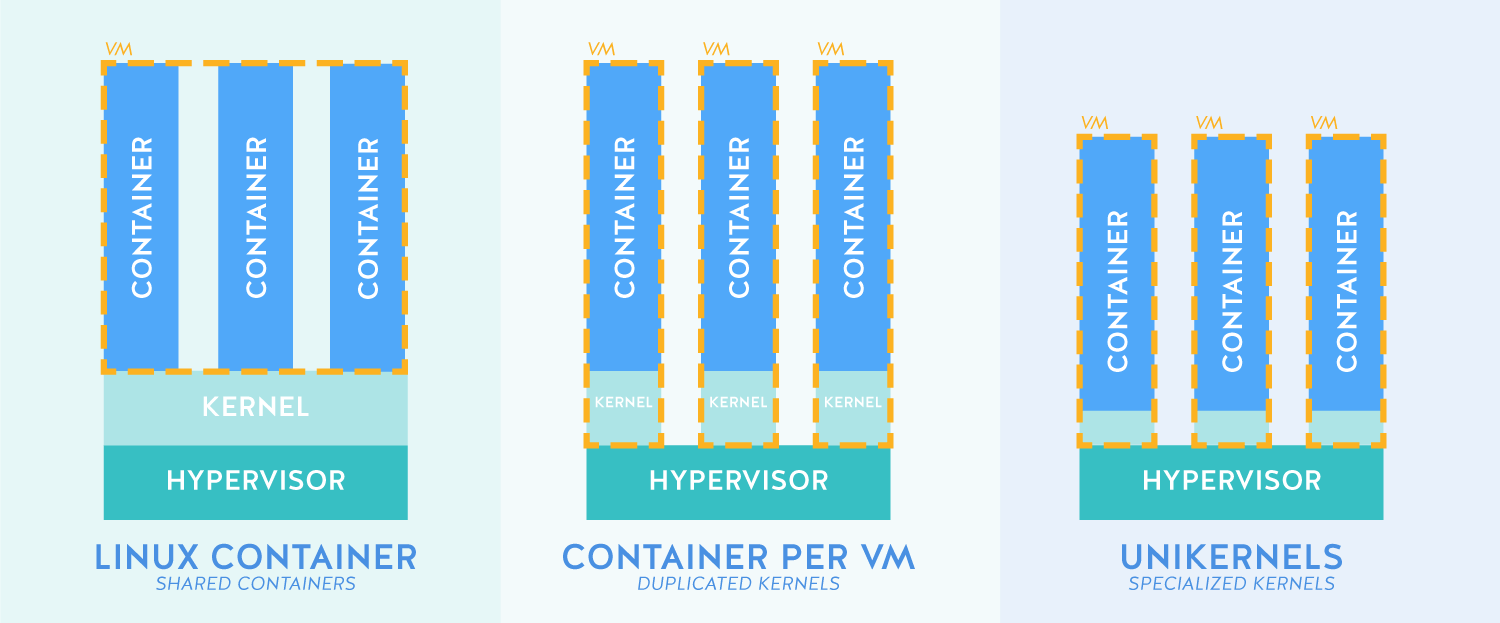
\includegraphics[width=0.8\textwidth]{figures/Linux-containers-vms-unikernels.png}
    \caption{Different virtualization techniques: https://nordicapis.com/introduction-to-unikernels/} \label{fig:virt}
  \end{figure}

  \section{Orchestration}

  \subsection{microservices}
\section{Managing IoT}
